%% $Id: surrey.tex,v 1.1 2006/01/30 21:12:09 pwaddell Exp $

\documentclass[12pt,a4paper]{article}

\usepackage{txfonts}
\usepackage[T1]{fontenc}
%\usepackage[latin1]{inputenc}

\usepackage{array}
%\usepackage{lscape}
\usepackage{rotating}
\usepackage{longtable}
\usepackage{lscape}
%\usepackage{natbib}
\usepackage{url}
\usepackage{graphicx}
\usepackage{supertabular}

%
% Change coordinates to edge of page
\voffset=-1in \hoffset=-1in
%
% Set for US Letter
\textheight=9.5in \textwidth=6.5in \topmargin=0.5in
\oddsidemargin=1in \evensidemargin=1in
%
\frenchspacing \raggedbottom
%\renewcommand{\thesection}{\Alph{section}}
%\renewcommand{\theenumii}{\arabic{enumii}}

%\newcommand{\ve}[1]{\mathbf{#1}}
\newcommand{\vk}[1]{\mbox{\boldmath $#1$}}
\newcommand{\tight}{\itemsep 0pt}

\begin{document}

\title{Confronting the Bane of Endogeneity in Modelling Urban Social Dynamics}

\author{\\
Workshop on Modelling Urban Social Dynamics\\\\
University of Surrey\\\
April 7-8, 2005\\
\\\\
Paul Waddell\\
Director, Center for Urban Simulation and Policy Analysis\\
Evans School of Public Affairs, University of Washington,\\
Box 353055, Seattle, WA 98195 \\
( 206) 221-4161, pwaddell@u.washington.edu} \maketitle


\baselineskip=.3in

\begin{abstract}
\baselineskip=.3in

The problem one quickly faces in developing a simulation model of
urban dynamics is that almost everything seems to be endogenous.
Household location choices, firm location choices, real estate
development choices, and governmental infrastructure and public
service choices all interact dynamically.  This paper describes an
evolving effort to represent key endogenous choice processes at an
agent level in UrbanSim, an operational urban simulation model
system designed to explore the potential effects of alternative
public policy choices.  Specific recommendations are developed to
refine simulation systems such as UrbanSim to more effectively
confront the endogeneity issues raised in the paper.
\end{abstract}
\clearpage

\section{Introduction}
Studying urban social dynamics is a long-standing preoccupation in
much of social science.  Modelling these dynamics has a shorter
history, but is motivated both by a desire to understand the
underlying processes of change, and by the desire to influence
them to ameliorate urban social, economic, or environmental
problems.  The range of theoretical and empirical frameworks to
analyze and predict urban dynamics is incredibly broad, and new
syntheses and hybrids emerge continuously.

What do we mean by urban social dynamics? In the context of this
paper, we interpret the term to mean intra-metropolitan
spatio-temporal changes in social and economic composition of
neighborhoods. Or, more explicitly, the evolving neighborhood
location patterns of households by type, and the causes and
effects of these changes. Processes and patterns of race and class
segregation, suburbanization, and gentrification fall within this
scope, as does housing development and redevelopment, housing
prices, firm location, and the provision by local governments of
infrastructure and public services.

The problem one quickly faces in developing a simulation model of
urban dynamics is that almost everything seems to be endogenous.
Considering that a model is intended to be an abstraction, a
simplification of reality to be used to better understand certain
aspects of it, we find that the first major challenge in model
development is determining in a satisfactory way where to draw the
boundary between what is to be modelled as endogenous behavior and
what is to be considered exogenous, and therefore not modelled
explicitly.  Although this interpretation of endogeneity presents
substantial difficulty for modelling, a second and perhaps more
insidious set of endogeneity problems arise within the scope of
the behavior that is modelled explicitly.

The objectives of this paper are to:

\begin{itemize}
\item  Summarize general requirements for modelling urban social
dynamics for the purpose of formative policy evaluation, and the
design responses made in the development of UrbanSim;

\item Identify key sources of endogeneity within urban social
dynamics, and examine the implications of these for model design;

\item Assess the current specification of UrbanSim to address
these endogeneity concerns, and develop strategies to improve the
treatment of these concerns.

\end{itemize}


\section{Urban Modelling and Formative Policy Evaluation}
The use of models to assist in the formation of policy has a long
tradition in the broad arena of urban policy.  Much of the early
work in the 1960's focused principally on transportation policy,
and led to the development of the precursors to current 4-step
travel demand model systems that are now a standard part of the
metropolitan planning process \cite{}. Models of urban development
using spatial interaction techniques came into moderately
widespread use in the 1970's, for predicting land use change
associated with transportation improvements
\cite{putman-book-1983}.  Other land use models were developed
around the same time that used a spatial extension of the
Leontieff Input-Output model of the U.S. national economy
\cite{echenique-transport-reviews-1990,delabarra-book-1995}. There
were high expectations in the early modelling projects that these
projects would rapidly change the policy-making process, making
urban models the centerpiece of urban policy.  Expensive projects
needed to be evaluated efficiently prior to making substantial
capital investments, and cost-benefit analysis was promoted to
assess the relative cost-effectiveness of alternative projects.

The design of early operational urban models was generally
aggregate in the representation of agents and geographies, and
cross-sectional in the representation of time.  They imposed some
form of iterative procedure to converge to a time-abstract
equilibrium, and assigned this to a specific year in the long-term
planning horizon for transportation projects, with no
path-dependence representing the evolution of the urban system
from the current to the predicted state.  In 1973, Douglas Lee
wrote "Requiem for Large-Scale Urban Models," a scathing critique
of the urban modelling efforts of the time
\cite{lee-1973,lee-1994}. This critique heavily influenced federal
attitudes towards investment in urban modelling research, and
helped to trigger an era of skepticism about their potential that
persisted for more than two decades.

Most of the criticism raised by Lee was well-founded.  The models
came to be known as `black-box' models because their behavior was
not at all transparent, they were unnecessarily complex and
abstract, and this significantly limited their effectiveness as
tools for communicating with policy-makers and the public about
policy alternatives.

Many things have changed regarding the environment for urban
modelling since Lee's critique in 1973, including a tendency to
forget the concerns he raised.  Much of the obvious change is on
the 'supply side' of modelling, or the capacity for
model-building. Computational capacity has dramatically increased,
information management in the form of database and Geographic
Information Systems has revolutionized data processing, data
available for fitting urban models has become more widely
available and more detailed, sophisticated statistical methods
have emerged, theoretical and empirical research on the underlying
processes has progressed, and new frameworks for microsimulation
and agent-based modelling at the individual level have appeared.

Other changes have come on the 'demand-side' of modelling, and
these have also heavily shaped recent modelling projects.  The
practice of urban policy development and planning has been
subjected to substantial pressure to become more transparent and
democratic, with greater public participation in all stages of the
policy process.  This pressure has met varying degrees of
responsiveness among public agencies, of course, but the pressure
is widespread.  Further, the nature of the questions being raised
in the policy process are increasingly diverse, and considerably
more complex than the civil-engineering oriented processes of the
middle twentieth century that focused on efficiently sizing
capacity to meet anticipated demand on the transportation system.
Questions of economic efficiency are now generally balanced in the
public discourse with concerns about social equity and
environmental health and sustainability, with widely varying
representation of these stakeholder interests from place to place.

The convergence of these supply-side and demand-side trends has
led to a resurgent interest in urban modelling for formative
policy evaluation. In 1995, a conference was convened by the
Travel Model Improvement Project of the Federal Highway
Administration to assess he state of urban modelling.  Many of the
recommendations echoed criticisms raised two decades earlier by
Lee, but there was also a clear sense of renewed enthusiasm in
developing new modelling approaches, and the ensuing decade has
generated a proliferation of modelling projects.

In the late 1990's, the development of UrbanSim  was begun as an
effort to create an operational urban modelling system that would
be a fundamental departure from the aggregate, time-abstract
models that had been the mainstream approach in operational urban
models, and which would respond to the above-mentioned changes on
the demand and supply side of modelling.  UrbanSim was intended to
promote a more open, participatory approach to formative policy
evaluation, so it emphasized behavioral transparency in its
design.  In keeping with an emphasis on transparency, it was
released as Open Source software, and has been continually updated
since its initial release in 1998.  It is available from
\url{www.urbansim.org}.

The emphasis on transparency led to a design focus on
representation of agents, their choices, and their dynamic
interaction over time. The intent was to make the modelling
reflect as transparently as possible the real world aspects the
model represented, so that communication about the model would
reflect as much as possible the syntax used to describe the real
phenomenon of interest: households and firms locating, real estate
developers developing and redeveloping real estate, and the role
of governments in creating transportation infrastructure that
influences accessibility and setting land use regulations that
constrain development.  The representation of policies, ranging
from transportation, to land use, to environmental, should be
explicit, and their effects on outcomes of interest manifested
through the sensitivity of the agents to changes in their
environment caused by these policies.  The resulting modelling
framework had several key design features
\cite{waddell-env-and-planning-2000,waddell-japa-2002}, all of
which have been subsequently promoted by others in the research
community as elements of an `ideal' model system
\cite{miller-tcrp-1999}:


\begin{itemize}

\item Agent-level representation: individual households and jobs

\item Dynamic representation of time, usually in annual steps,
with path-dependence

\item Representation of highly disaggregate geographies, such as
small grid-cells or parcels

\item Representation of individual choice processes: moving,
locating

\item Use of a discrete-choice modelling framework to represent
choice behavior.

\item Representation of interactions of households, firms and
developers in real estate markets, and the role of prices.

\item Representation of \emph{scenarios} of public policies for
land use, transportation and the environment .

\end{itemize}

UrbanSim models household residential location choice, employment
location choice, and real-estate development choice models as
discrete choice models, drawing on the Random Utility Maximization
(RUM) framework pioneered by Daniel McFadden, who won a Nobel
Prize in Economics for this and related work
\cite{mcfadden-1974,mcfadden-1981}. For each agent, we assume that
each alternative $i$ has associated with it a utility $U_i$ that
can be separated into a systematic part and a random part:
\begin{equation}
    U_i = u_i + \epsilon_i,
    \label{eq:utility}
\end{equation}
where $u_i = \vk{\beta}\cdot\vk{x}_i$ is a linear-in-parameters
function, $\vk{\beta}$ is a vector of $k$ estimable coefficients,
$\vk{x}_i$ is a vector of observed, exogenous, independent
alternative-specific variables that may be interacted with the
characteristics of the agent making the choice, and $\epsilon_i$
is an unobserved random term. Assuming the unobserved term in
(\ref{eq:utility}) to be distributed with a Gumbel distribution
leads to the familiar multinomial logit model
\cite{mcfadden-1974,mcfadden-1981}:
\begin{equation}
    P_i = \frac{\mathrm{e}^{u_i}}{\sum_j \mathrm{e}^{u_j}},
    \label{eq:mnl}
\end{equation}
where $j$ is an index over all possible alternatives. The
estimable coefficients of (\ref{eq:mnl}), $\vk{\beta}$, are
estimated with the method of maximum likelihood (see for example
\cite{Greene-2002}).

Within the UrbanSim model system, the choice process proceeds as
shown in Figure \ref{fig:choiceprocess}.

\begin{figure}[h]
\center
 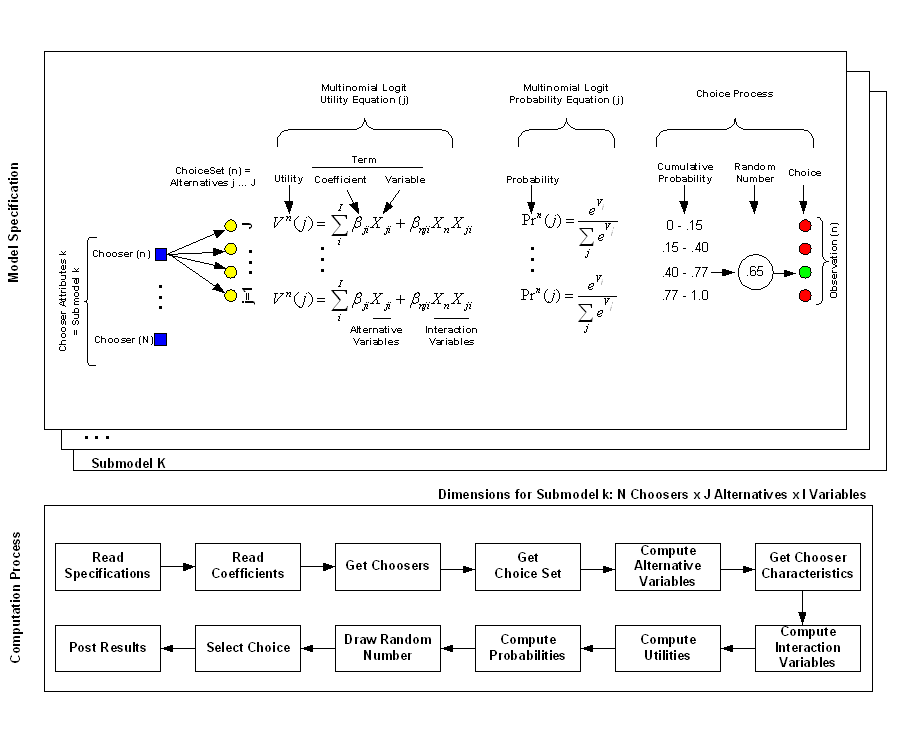
\includegraphics[width=6.5in]
 {ChoiceProcess.png}
\caption{Choice Process in UrbanSim Location Choice Models}
\label{fig:choiceprocess}
\end{figure}

The first steps of the model read the relevant model
specifications and data.  Then a choice set is constructed for
each chooser.  Currently this is done using random sampling of
alternatives, where alternatives are grid cells of 150 meters by
150 meters, and the cells are weighted by the number of locational
opportunities in them (vacant housing for the residential location
choice model).  Note that this sampling method has been shown to
generate consistent, though not efficient, estimates of model
parameters \cite{ben-akiva-lerman-1987}.

Once the choosers (movers or new households) are selected and the
choice sets of alternative locations sampled, the relevant
variables used in the utility function are computed.  For
efficiency, this proceeds by computing characteristics of
alternatives first for all alternatives in the universe, then
computing interaction terms for only the set of choosers and their
sampled locations.  After this, the logit calculations predict
probabilities for all the available choices in the choice set for
each chooser.  Finally, the process makes a selection by drawing a
random number, comparing it to the cumulative distribution of the
predicted alternatives, and selecting the choice which the random
draw falls within.  At this point the choice is posted to the
database for the chooser, and the number of available housing
units is reduced by one to reflect that the unit is no longer
vacant.

Household agents have characteristics of race, income, size,
presence of children, age of head, number of workers, and number
of vehicles. The initial base year population is derived from
census data using a synthetic population procedure
\cite{beckman-1995}, which uses Iterative Proportional Fitting to
scale the joint probability distribution of household
characteristics in the Census Public Use Microdata 5\% Sample to
the marginal distributions available by census tract and block
group from Census Summary File 3. A sample of real households is
used for model estimation, generally taken from regional surveys
for transportation planning.  These surveys provide detailed
geocoding to allow assignment of locational characteristics to
sample households, which is essential for estimating location
choice models.

Firms are represented in UrbanSim at the level of individual jobs,
with the sector of the firm and the location of the establishment.
Typically, public sources of employer data from unemployment
insurance records have been used to generate an inventory of
business establishments for model application.

Information on individual land parcels is obtained from individual
tax assessor offices and compiled into a regional database.
Considerable imputation and cleaning of these data are often
needed, to address gaps and inconsistencies in the data, such as
tax-exempt properties.  The attributes generally include year of
construction, type of development, square footage of building,
land area, land use classification, and land and improvement
(building) values.  These data are then transformed into a grid
representation for model development purposes, combining parcel
fragments that fall into the same grid cell and assigning an
overall development type classification to the cell.  Quantities
of housing and nonresidential square feet are retained for
accounting of occupancy by households and jobs.  A detailed
discussion of the data integration process is available
\cite{waddell-cuspa-2004}.

The need to run the model in operational contexts ranging from
small to large metropolitan regions, and representing individual
households, jobs and small grid cells, led to significant
challenges in the software design and implementation.  Java was
used as the development language, but its object overhead required
too much memory to scale well to larger regions on standard
desktop computers.  To address this, a design of exploded objects
was used to retain an object representation, but using an internal
storage mechanism of parallel arrays.  Another key design element
in the software architecture was the use of implicit invocation to
manage communication by modular model components entirely through
their interaction with a data store \cite{noth-ceus-2003}.  In
addition to these techniques to improve efficiency, substantial
caching was used to avoid redundant computing.

UrbanSim has now been applied in several metropolitan regions,
including Eugene-Springfield, Oregon, Honolulu, Hawaii, Houston,
Texas, Salt Lake City, Utah, and Seattle, Washington, and has been
validated longitudinally by comparing 15 years of path-dependent
simulation to observed outcomes \cite{waddell-japa-2002}.  Several
more metropolitan areas are in the early stages of applying the
model system in the U.S., such as Denver, Colorado and Detroit,
Michigan, and abroad, including Amsterdam, the Netherlands, Paris,
France, and Z\"{u}rich, Switzerland.


\section{The Bane of Endogeneity}


\subsection{Endogenous Modelling Scope}

The problems motivating this paper are ones arising from the high
degree of endogeneity in the urban system we are modelling. The
first concern in model design is determining the scope of the
model, or the boundary between those processes to be considered
endogenous to the model and those to be treated as exogenous to
it.  In our application, we are concerned with analyzing the
effects of public policies addressing infrastructure, housing,
urban development, and environment within a particular study area
defined as a metropolitan area, typically based on official
designations for transportation planning purposes. These policies
draw focus to household and firm location and travel, to real
estate development, and markets as interacting components of a web
of causation.  One notable aspect of this web is that the choice
processes related to travel, residential location choice, real
estate development, and infrastructure construction vary
tremendously in temporal scale, as noted in Figure 1.

\begin{figure}[h]
\center
 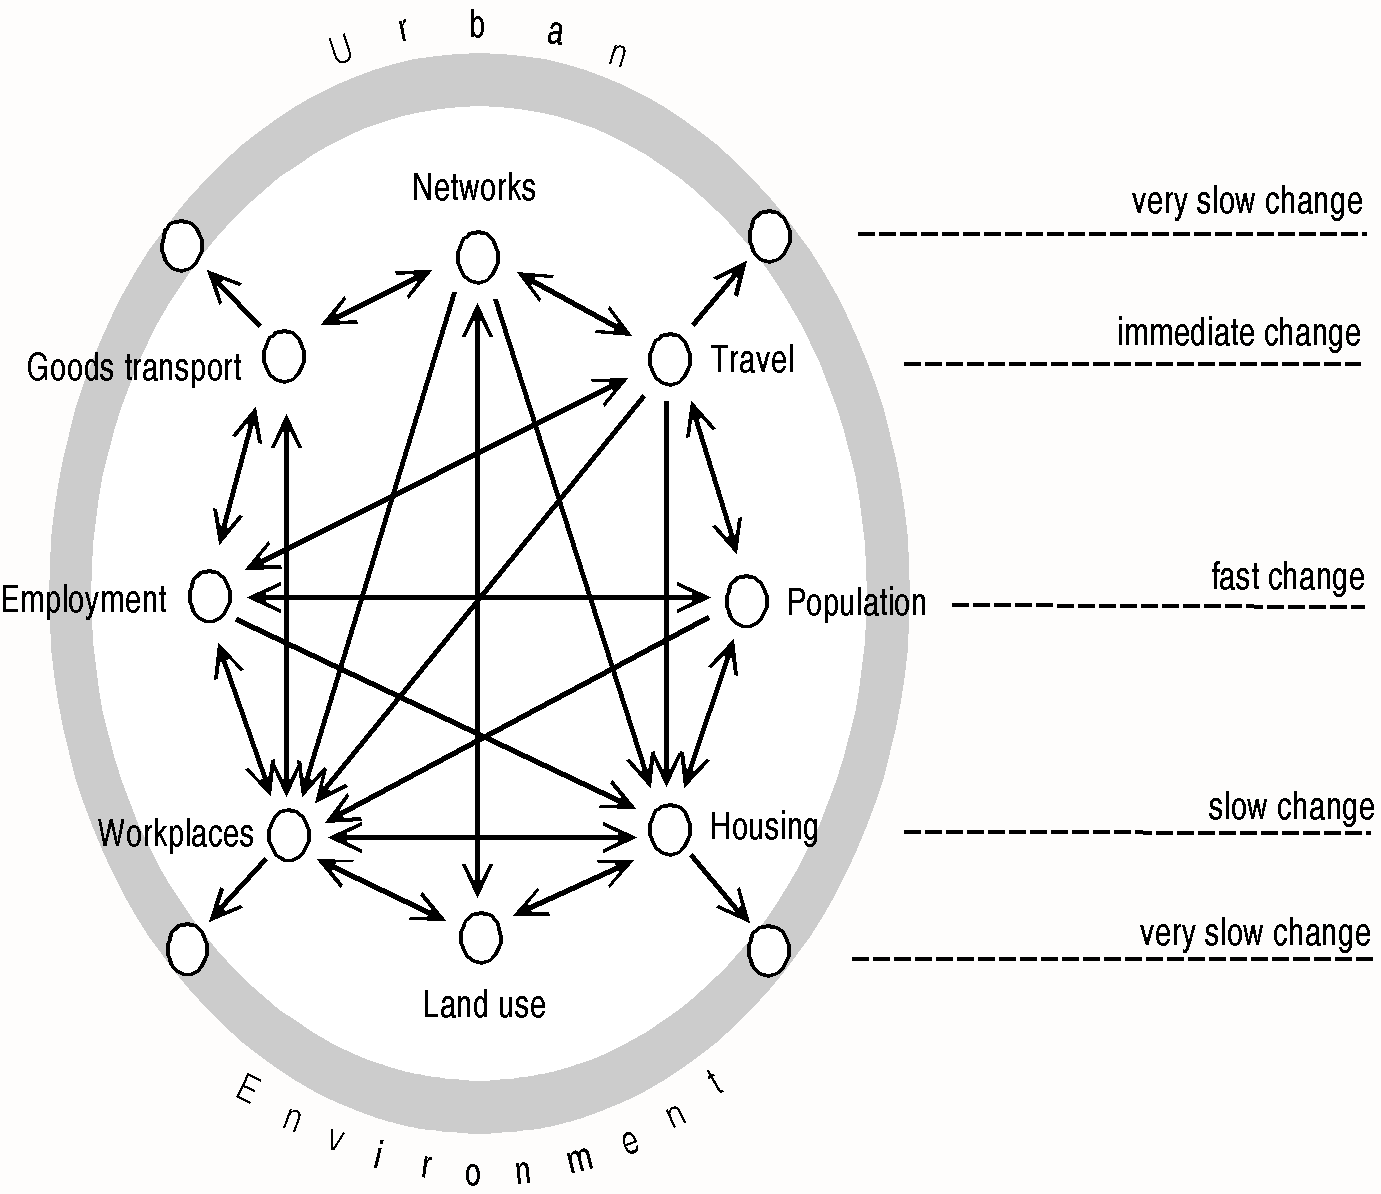
\includegraphics[width=4.5in]
 {wegener.png}
\caption{Web of Urban Processes, from \cite{wegener-1994}}
\label{fig:wegener}
\end{figure}

For the purposes outlined earlier in the paper, the scope of
engodeneity is well represented in Figure \ref{fig:wegener}. These
processes are the central ones in focus, and other processes are
implicated only as needed to adequately represent these.

It is likely that failure to represent almost any of the nodes in
this Figure will induce a significant degree of endogeneity bias
with respect to evaluating urban policies that deal with any of
the nodes.  That is to say, if we assume any of the nodes to be
exogenous, and either leave it out of the model entirely (a gross
misspecification) or assume it is not influenced by feedback from
other nodes we are considering, then our conclusions are
potentially significantly biased by this omission. For a thorough
explanation of the statistical properties of endogeneity bias and
methods to test for the presence of such bias in standard
statistical models, see Greene's treatment of the subject
\cite{greene-2002}.

In the development of UrbanSim to date, the transportation
components represented in the figure are included by loose
coupling to an external travel model system, and the
specifications of the travel model depend on the particular
metropolitan area.  It is common in current-generation
transportation models that goods transport is poorly incorporated
or not included at all, raising a potential source of bias.  This
may be one of the most innocuous of the sources of endogeneity
bias, as others addressed below are likely to have a greater
distorting effect on system behavior.

To address the complexity of the endogenous processes and their
interactions, we have taken into consideration the time scales of
the process to partition processes.  Travel behavior is modelled
(by a loosely coupled travel model system) as a within-day set of
processes, which treat the spatial distributions of activities and
real estate as exogenous, or fixed for the period of the day.
Similarly, we model the location choices of households and firms
within a period we refer to as the short-term (typically defining
this to be more than one day but less than one year).  Short-term
processes treat long-term processes (anything more than a year) as
exogenous - which means the supply side of the real estate market
operates at a long-term scale, while the demand-side operates at a
short-term scale.  Processes that occur within the short-term are
separated from each other by imposing an assumption of limited
information, myopic behavior.  In other words, we avoid the
assumption that agents each know what all other agents are going
to do in the short-term, and optimize their choices based on a
competitive game.  Nor do we impose the assumption that all
processes arise from individual agent-agent interactions. Instead,
we assume that agents make individual choices using limited
information from the past period to form their expectations about
the present and future. These temporal-partitioning and myopic
information assumption allows the model system to be constructed
in a very modular way, minimizing the need for individual
agent-agent interaction or perfect foresight assumptions. These
assumptions (and other design choices) distinguish the UrbanSim
modelling approach from those used in most multi-agent simulation
frameworks such as SWARM, RePast, Ascape and other multi-agent
systems.


\subsection{Endogenous Modelling Boundary}
The spatial extent of the processes considered endogenous is
determined fairly imperfectly based on planning area boundaries
that tend to use official building geographic blocks such as
Counties, and group these into metropolitan regions based on the
degree of social and economic integration, as evidenced in
commuting patterns.  In an ideal situation, the study area
boundary would clearly differentiate one metropolitan study area
from another.  Clearly there are many cases that seriously violate
the assumption that the area outside the boundary does not
significantly influence the internal processes within the study
area.  Almost any metropolitan area on the eastern coast of the
United States, and most in western Europe, are close enough to
each other that the degree of commuting and economic exchange
among them is quite high.  This is the first major endogeneity
bias we must confront.

As the design of UrbanSim is focused on the spatial processes
within a metropolitan region, the boundary effects caused by
metropolitan spillovers surfaces a larger problem, which is that
macro-scale processes are currently handled by loose-coupling to
macro-economic models, but only in the direction from macro-scale
to micro, and not in the reverse direction. This means that local
processes cannot induce changes in the macro-economy, a
potentially significant omission. In particular, it means that two
kinds of policy effects are not currently possible to measure, by
construction.  First is the aggregate economic effect of a major
infrastructure project or other policy. Some of these projects are
arguably large enough to induce measurable macro-scale effects,
such as a new airport. Others, such as localized zoning policies,
would be quite unlikely to induce macro-scale effects on economic
growth.  Second, some policies such as urban growth boundaries or
impact fees have been argued in the literature to potentially
produce enough inflation in housing prices to induce businesses
and households to consider alternative metropolitan locations.  If
there are other metropolitan areas within plausible commuting
distance, this could produce a measurable displacement and trigger
increases in between-metropolitan travel.

How significant this source of endogeneity bias is, and whether it
is large enough to seriously distort the conclusions of an
analysis of local land use, transportation, or environmental
policies, is an open research question.  Certainly, if possible,
it should be addressed in further refinement of the model system,
but it will require integrating macro-scale processes and their
interaction with surrounding metropolitan areas.  We will leave
this particular area of further development to a future paper.

\subsection{Endogenous Market Clearing and Prices}

A major endogeneity issue arises in the context of location
choice, due to the need to reconcile the choices made by locating
agents with the fixed available supply of real estate at those
locations. We shall refer to this in general as a \emph{market
clearing} process, but only in the limited sense that we impose
the accounting constraint that once a location (housing unit) is
chosen by an agent, it is occupied and not available to another
agent until it is vacated by the first.  This means that there
will often be a scarcity of housing at more desirable locations,
and there must be some means to ration the scarce housing among
the agents that wish to locate in them. The assumption of a fixed
supply (stock) of housing in the short-run is equivalent to
assuming that if a household is looking for a house this month,
they cannot contract to have a house built and made available for
them next month.  The time frame for housing supply, as noted
earlier, is considerably longer than the time scale for
residential location choice.

The process currently used in UrbanSim, described in Figure
\ref{fig:choiceprocess}, deals explicitly with the market clearing
constraint imposed by having a fixed supply of housing in the
short-run time frame in which households are making a location
choice.  The market clearing process as currently modelled assumes
that the scarcity of housing at any given location is rationed
according to a randomized order, first-come-first-served process,
not unlike a lottery for the available houses.  It is certainly
not difficult to draw on experience to confirm that there is a
strong degree of random, but sequential, dependence in the way the
housing market works. If person A arrives first and makes a
successful bid on a house, it is not available to person B, even
if the latter would be willing to pay more.

A visual example of the current algorithm makes the process
clearer. Let us simplify the situation to one in which there are
16 neighborhoods, arranged in a rectangular grid.  Assume that
they have 10 houses in each and that there are exactly 160
identical households looking for housing.  Assume further that the
attractiveness of the neighborhoods varies in a systematic way:
cells in the corners have the least attractiveness (1), those on
the edge and not in the corners have an attractiveness of (2), and
those in the center have the highest attractiveness (3).  Note
that the utility is defined as the exponentiated value of these
attractiveness terms, and it is the relative utility that directly
influences choice probabilities.

Figure \ref{fig:grid1} below shows the attractiveness (a), sums of
the individual choice probabilities (b), the count of choices made
by this sample of 160 households on this particular draw of random
numbers \footnote{Note that with a relatively small number of
observations the sum of the choice probabilities differs
significantly from the choice counts due to simulation randomness.
This simulation error diminishes as the number of observations
increases.} (c), and the excess demand in those cells that the
counts exceed housing supply (d).  The excess demand would be the
number of households forced to make a second-best choice from the
remaining available housing, and this would proceed until all
households are placed, provided that there is available housing.
In this example, it would mean that each cell would end up with 10
households, though many would have preferred to locate in the
center cells.

The endogeneity concern in market clearing is twofold.  First,
even though housing prices are included in the utility function,
they are updated only between one simulation year and the next,
and do not dynamically change during a simulation year.  This
places all of the burden of rationing the scarce housing supply
within a simulation year on the lottery process described here,
which may not give enough weight to the role of competitive
bidding in a tight housing market.  On the other hand, it is not
apparent that the market works as a perfectly-informed and
efficient instrument, either. It is implausible to assume that all
households participate in a single massive auction, and each
obtains the house they most prefer, subject to budget constraints,
in a competitive bidding process.  It is more likely that the
random arrival and bidding processes are both facets of the actual
operation of the market.

\begin{figure}[h]
\centerline{
 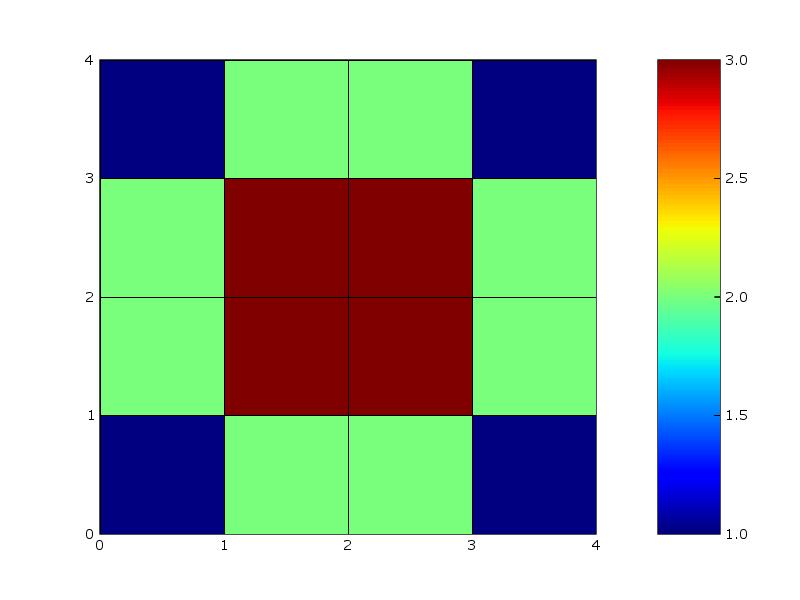
\includegraphics[width=.45\textwidth,height=0.35\textwidth]
 {example_grid_util.png} \hspace{1cm}
 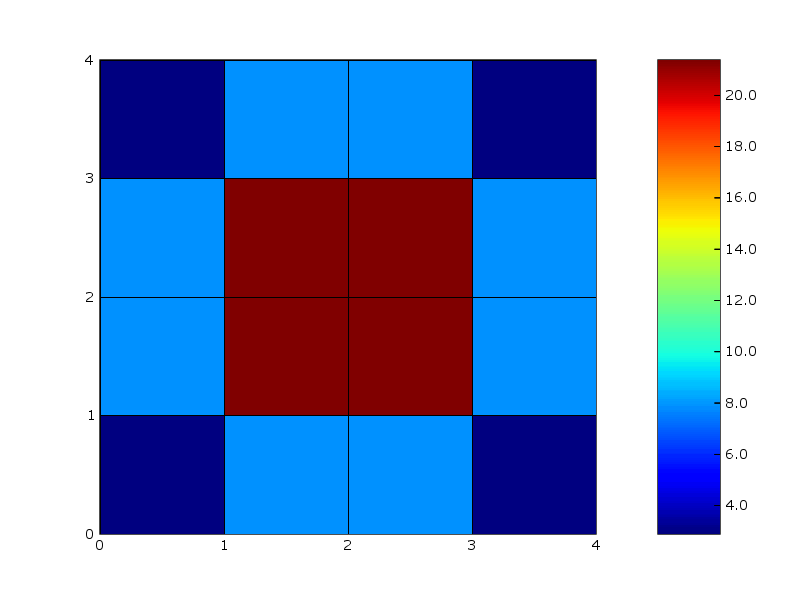
\includegraphics[width=.45\textwidth,height=0.35\textwidth]
 {example_grid_prob.png}}
\end{figure}

\begin{figure}[h]
\centerline{
 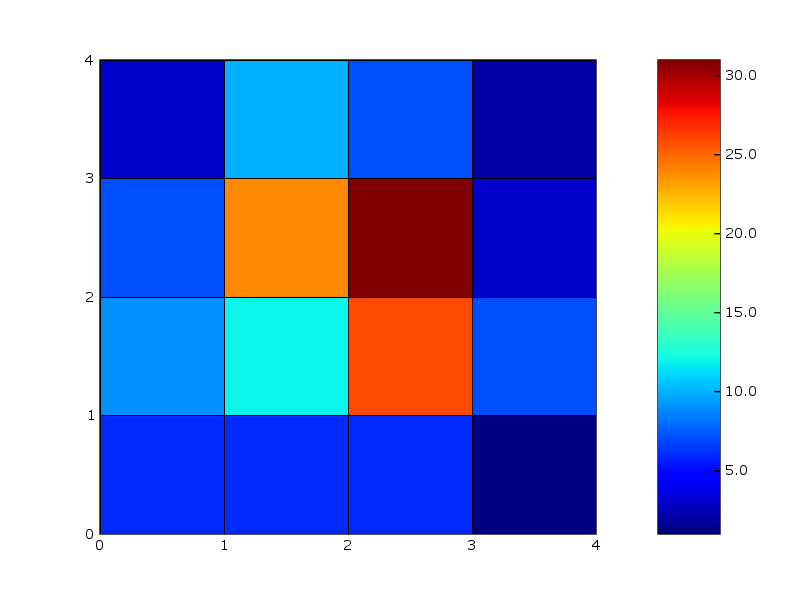
\includegraphics[width=.45\textwidth,height=0.35\textwidth]
 {example_grid_count.png} \hspace{1cm}
 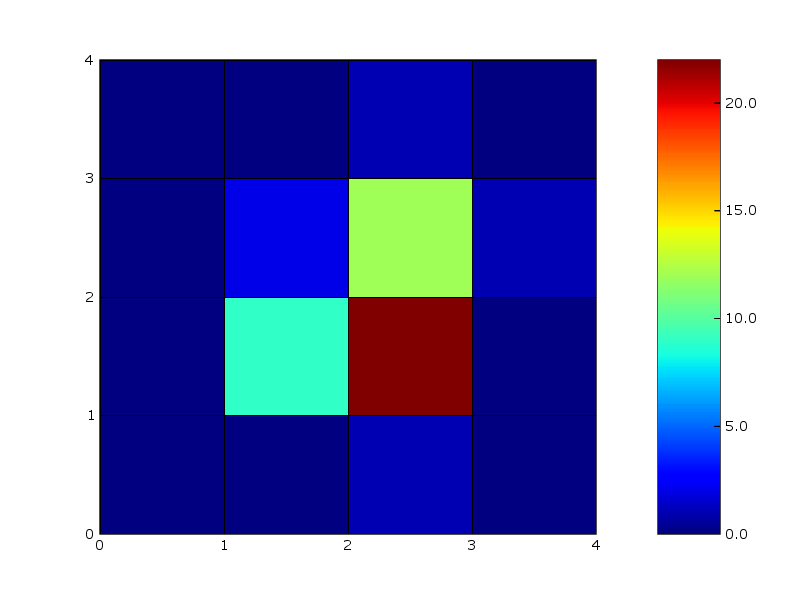
\includegraphics[width=.45\textwidth,height=0.35\textwidth]
 {example_grid_excess.png}}
\caption{\label{fig:grid1} Choice Model Predictions With Limited
Housing}
\end{figure}

\begin{tabbing}
------- \= ------------------------------------------------------------ \= \kill
\> (a) Attractiveness (log(Utilities))  \> (b) Sum of
Probabilities \\  \> (c) Choices (among 160 choosers) \> (d)
Excess Demand
\end{tabbing}


To address these concerns we propose to modify the choice
algorithm shown in Figure \ref{fig:choiceprocess} in two ways. The
first is to simulate the role of a 'landlord' agent in each
neighborhood who monitors market conditions and attempts to
maximize profit by adjusting prices. Depending on how elastic the
demand is, due to substitution possibilities among alternative
neighborhoods, a landlord would increase prices in the presence of
multiple offers in order to increase profit, and lower prices if
the number of offers falls well below the number of housing units
available in the neighborhood.  This would be implemented as an
iterative loop at the choice stage, with landlords updating prices
to improve profits, and households altering their choices in the
face of modified prices.  Notice that both of these agent
responses are consistent with expected behavior, intuitively and
theoretically, and both work to restore balance between demand and
supply.  The revised algorithm is shown in Figure
\ref{fig:choiceprocess2}.

\begin{figure}[h]
\center
 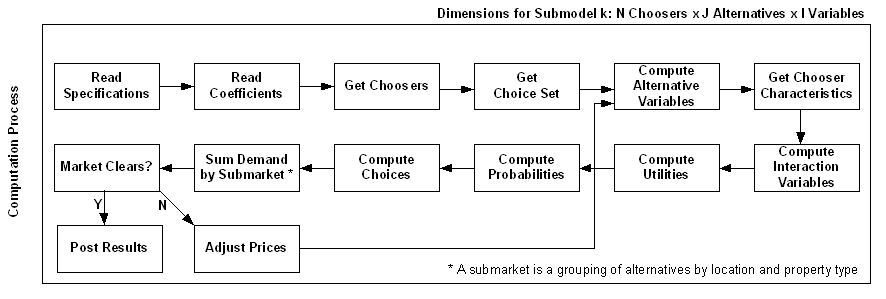
\includegraphics[width=6.5in]
 {ChoiceProcessWithPriceAdjustment.png}
\caption{Choice Process in UrbanSim Location Choice Models}
\label{fig:choiceprocess2}
\end{figure}


The second proposed change is to add a method to the algorithm to
allow the relative weight of the price adjustment process and the
lottery process to vary depending on parameters derived from model
calibration against observed data.  It should be possible to avoid
imposing an arbitrary assumption that only the price mechanism or
only the lottery mechanism are at work, and it should also be
possible to learn the mixture of these processes by examining
observed data.  This modification will require a respecification
of the logit model to include both a constraint and a price
effect.


\subsection{Endogenous Neighborhood Composition}
The literature on residential location choice contains several
streams of research on aspects that link the choices made by
individual households to the aggregate spatial patterns that
emerge.  The feedback between the aggregate patterns and the
individual choices is a major endogeneity concern in most of this
literature.  If the social composition of a neighborhood selection
is valued by a locating household, and the outcome of their
residential location choice changes the social composition of the
neighborhood they locate in, then the individual choice process
and the neighborhood composition are endogenous.

One approach to this endogeneity was first developed by Thomas
Schelling \cite{schelling-1969,schelling-1971,schelling-1978}.
This approach and its extensions simulates the relocation choices
of individual agents based on their satisfaction with the social
composition in their localized neighborhood. Schelling's early
model of residential segregation has inspired considerable
extension in the multi-agent simulation literature.  Its
attractiveness, and the attraction of more recent work on this
approach, derive in no small measure from its transparent
simplicity.  The utility function is essentially due to a single
factor, there are no costs to changing locations, and no
constraints on doing so.

Adding complexity to the utility function, and imposing accounting
constraints on housing supply and a market clearing process as
discussed in the preceding section would makes this modelling
approach considerably less elegant, and possibly less informative.
More problematic from a practical perspective is that there is
considerable computing overhead to processing all agent choices as
localized interactions of agents.  Scaling the model from a small
hypothetical situation to modelling metropolitan regions the size
of Paris, with 11 million inhabitants, or even Seattle, with 3
million, would not be practical on generally-available computers.
Last, it seems likely that localized interactions are insufficient
to capture the rich variety of information flow that informs agent
choices.  Information about housing market opportunities for
example may come from a newspaper or web site, personal experience
such as seeing a for sale or rent sign while travelling through a
neighborhood, information from a social network, or from a real
estate broker.

The approach we have used in UrbanSim to model endogenous
neighborhood composition is to include in the utility function
interaction terms between household characteristics and social
characteristics of the location, and to use a sample of recent
movers to estimate the household location choice model.  The
household characteristics used in UrbanSim include race, household
income, age of head, presence of children, number of persons,
number of workers, and number of vehicles.  Since the model uses
full enumeration of the households, generating compositional
measures using these characteristics is straightforward. What is
less straightforward is the choice of which interaction terms to
include in the utility function, and what spatial frames to use
for the measurement of the social composition effect.  To date,
only a small subset of the possible interaction terms have been
tested in the model system, though the framework and data exist to
test any of the others.

The spatial frame for measuring effects is challenging because of
the theoretical and empirical limitations in our understanding of
neighborhoods and neighborhood effects.  It is clear that defining
neighborhoods is a problematic exercise, since residents often
disagree about or do not know the boundaries of their
neighborhoods, and that the frames of reference differ depending
on the issue at hand: for example shopping for groceries or
choosing a high school.  Moreover, the use of fixed-boundary
neighborhoods can give rise to boundary problems and to potential
for the Modifiable Aerial Unit Problem (MAUP)
\cite{openshaw-taylor-1981}.

For these reasons, we have opted to make the selection of spatial
frames of reference as flexible as possible, using grid cells as
the low-level spatial building block. Figure \ref{fig:gridmap}
shows the relative scales of 150 meter grid cells in central
Seattle to Traffic Analysis Zone (TAZ) and Forecast Analysis Zone
(FAZ) geographies used in transportation modelling, and to
underlying land ownership parcels.  The spatial frames of
reference available in UrbanSim to measure compositional effects
are the following:

\begin{itemize}

\item Grid cell (user-definable, but typically 150 by 150 meters)
\tight

\item Radius Surrounding Grid Cell (user-definable, typically 600
meters)

\item Traffic Analysis Zone (used in transportation modelling)

\item Census Block, Census Block Group, or Census Tract

\item City

\item County

\item Any Geography that is Assigned to Gridcells

\item Dynamically Updated Boundaries Assigned to Gridcells
\footnote{The use of statistical classification techniques to
generate typologies of neighborhoods is being explored in
UrbanSim, but currently requires some coding to implement.}

\end{itemize}


\begin{figure}[h]
\centerline{
 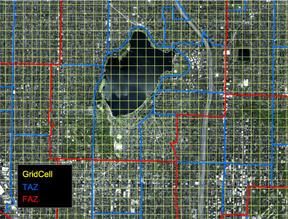
\includegraphics[width=.45\textwidth,height=0.35\textwidth]
 {gridmap2-small.png} \hspace{1cm}
 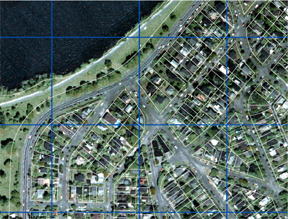
\includegraphics[width=.45\textwidth,height=0.35\textwidth]
 {gridmap-small.png}}
\caption{\label{fig:gridmap} 150 x 150 Meter Grid Cells in Central
Seattle}
\end{figure}

Compositional variables may be used at different scales, depending
on the nature of their effects, and there is no restriction on the
mixing of multiple scales.  This opens the possibility for
developing multi-level models that address the correlations among
multiple scales.  See for example, \cite{goldstein-book-1995} for
a thorough introduction to this topic.

In the application of UrbanSim in the Puget Sound region of
Seattle, Washington, the household location choice model was
estimated using a stratification of households by age and size, to
allow measurement of life cycle effects on the preferences of
households for locational characteristics.  Income and presence of
children were also used in the specification, but as interaction
terms.  Variables used in the Puget Sound household location
choice model are defined in Table \ref{tab:vardef}.  Model
estimation results using a sample of 2,364 households who moved
between 1995 and 2000 are given in Table \ref{tab:hlc}.

\begin{table}[h]
\caption{Variables Used in Household Location Choice Model, Puget
Sound Region} \label{tab:vardef}
\centering
\begin{tabular}{ll}
\hline\hline
BCOS\_IN & Annualized Cost of Housing / Household Income \\
BDUR\_C & Dwelling Units in Cell * Has Children Dummy \\
BART & Close to Arterial Dummy \\
BINCIVAL & Income * Improvement Value per Unit \\
BLDUW & Log of Dwelling Units within 600 Meters \\
BPHIW\_H & High Income Dummy * Pct High Income in 600 Meters \\
BPMIW\_M & Middle Income Dummy * Pct Middle Income within 600
Meters \\
BPLIW\_L & Low Income Dummy * Pct Low Income Within 600 Meters
\\
BPMNWMJ & Minority Dummy * Pct Minority Within 600 Meters
\\
BPMNWMN & White Dummy * Pct Minority Within 600 Meters \\
BSAGEFAZ & Number of Households in FAZ of Same Age Category as
Household \\
SSIZFAZ & Number of Households in FAZ of Same Size Category as
Household \\
BYH\_HDR & Young Household Head (< 40) * High Density Residential
\\
YH\_M & Young Household Dummy * Mixed Use \\
BHBWUSO & Utility of Travel to Work by Auto \\
BHBWUTW & Utility of Travel to Work by Transit \\

\hline
\end{tabular}
\end{table}

The cost to income ratio provides an interaction that captures
price effects on location choice.  It is expected have a negative
sign, meaning that households prefer spending a smaller fraction
of their income on housing if presented with two alternatives that
are the same on all other measured characteristics except cost.
The results are all negative, and significant for all except young
single-person and 3+ person households.

The interaction of income of household with the percentage of
households of the same income tercile within the area within
walking distance (600 meters) are significant and positive for
only 6 of the 18 parameters estimated (3 parameters for 6 types of
households), with the strongest positive effects for younger
households with 3 or more persons.

The interaction between minority households and the percent
minority within walking distance was positive for all but young
one-person households, and significant for all households with at
least 2 persons.  White households had negative and significant
coefficients on the percentage minority within walking distance in
all six household types.

Age clustering was tested with the same age in FAZ (a proxy for
larger neighborhood) but found to be significant only for young
singles, not an entirely surprising result.  Younger households
and those without children also showed quite different preferences
for urbanization, as measured by transit utility and density of
housing in a cell, with a greater affinity to areas with high
transit utility and higher density.

The interactions of household characteristics and social
composition of neighborhoods, measured at scales from the grid
cell, to walking distance, to larger FAZ geographies, measure the
degree to which neighborhood composition influences individual
choice of residence location.  After households make choices and
locate in specific cells over the course of an annual simulation
step, the composition of each neighborhood is updated, and these
new compositions influence choices in the subsequent year. This
process represents the feedbacks between individual choice and
neighborhood composition, but there is still considerable room for
improvement.

One of the first improvements that can be made is to address the
market clearing endogeneity concerns outlined in the preceding
section, as these will interact with the neighborhood composition
concerns.  For example, if the current algorithm relies
unrealistically on a lottery process for market clearing, it is
likely to cause excessive diffusion in spatial concentrations of
social groups over time.

Two potentially confounding specification issues that warrant
further investigation are the role of taste heterogeneity and of
unmeasured quality variations that are correlated with price.  In
a stream of research pioneered by Berry, Levinsohn and Pakes in
1995, there has been a growing body of research dealing with the
specification and estimation of choice models with unmeasured
quality and taste heterogeneity
\cite{berry-econometrica-1995,berry-cowles-2003}. Initially
focused on the automobile market, this research has recently
expanded to address the housing market, neighborhood sorting and
segregation
\cite{bajari-kahn-stanford-working-papers-2002,bayer-mcmillan-rueben-2003}.
It suggests that failure to account for taste heterogeneity and
unmeasured quality variation correlated with price could bias
parameter estimates significantly. Testing these specification
concerns in the context of UrbanSim remains for future research.


\section{Conclusions}

Endogeneity is a serious challenge to successful modelling of
urban social dynamics.  In the design of UrbanSim we have
addresses with reasonable success the treatment of engogeneity of
modelling scope, particularly through the decoupling of processes
that run at different time scales, but also by using assumptions
about information that are neither entirely local, nor perfectly
informed about the present and future.  Endogeneity of modelling
boundary has been handled only indirectly by delegation to a
loosely-coupled macro-economic model, but this is not completely
satisfactory as it is only a top-down feedback now.  Future work
should address this limitation.

The two sources of endogeneity dealt with in more detail are those
associated with location choice, endogeneity of market clearing
and endogeneity of neighborhood composition. Regarding the first,
there is clearly a need to balance the roles of random aspects
that arise from random sequencing of location choices with the
role of price adjustment through a competitive process or a
supply-side (landlord) adjustment.  These need further development
in future research.  Regarding the second, much has been done
already to incorporate neighborhood composition effects, at
multiple levels, with and without fixed boundaries.  More remains
to be done, especially by exploring specifications that allow for
measuring taste heterogeneity and unmeasured quality variations
that are correlated with price, which could cause endogeneity
bias.

One of the main steps being taken to facilitate these next
advances is the re-engineering of the UrbanSim software platform.
It is being ported from Java to Python, using numeric libraries,
to increase speed, modularity, and productivity in code
development.  A broad international group of research teams is
beginning to collaborate around the development of this platform,
under the working name of Open Platform for Urban Simulation
\footnote{A preliminary website has been set up to provide access
to software developed by the project, and the first release is
expected some time in 2005.  See www.opus-network.org}.

\vspace{1cm} {\bf \large Acknowledgments}

The research described in this paper has been funded principally
by grants from the National Science Foundation Grants EIA-0121326
and BCS-0120024, and the Puget Sound Regional Council.

\clearpage
\begin{table}[h]
\caption{Estimation Results for Household Location Choice Model,
Puget Sound Region} \label{tab:hlc} \centering
\begin{tabular}{lrr|rr|rr}
\\
Age 40 or Less  &   \multicolumn{2}{c}{1 Person}  &
\multicolumn{2}{c}{2 Person}   &   \multicolumn{2}{c}{3 or More Persons}    \\
\hline\hline & beta & b./std. err & beta & b./std. err & beta &
b./std. err \\
BCOS\_IN &   -0.2557 &   -1.63   &   -1.7230 &   -4.74   &   -0.1572 &   -1.20   \\
BDUR\_C  &       &       &   -0.0122 &   -2.24   &   -0.0111 &   -5.14   \\
BART    &   0.2072  &   1.44    &   0.0684  &   0.49    &   -0.1166 &   -1.00   \\
BINCIVAL    &   0.0000  &   1.28    &   0.0000  &   5.54    &   0.0000  &   6.36    \\
BLDUW   &   0.3763  &   3.18    &   0.2172  &   2.08    &   0.2857  &   4.16    \\
BPHIW\_H &   0.0381  &   2.66    &   0.0080  &   0.81    &   0.0144  &   2.07    \\
BPMIW\_M &   0.0164  &   1.59    &   0.0166  &   1.76    &   0.0267  &   4.19    \\
BPLIW\_L &   0.0214  &   2.50    &   -0.0016 &   -0.14   &   0.0185  &   2.34    \\
BPMNWMJ &   -0.0021 &   -0.18   &   0.0312  &   2.50    &   0.0225  &   2.39    \\
BPMNWMN &   -0.0152 &   -2.58   &   -0.0188 &   -3.12   &   -0.0182 &   -3.80   \\
BSAGEFAZ    &   0.0005  &   3.66    &   0.0002  &   1.67    &   0.0000  &   0.29    \\
SSIZFAZ &   -0.0001 &   -1.68   &   0.0000  &   -0.27   &   0.0002  &   1.87    \\
BYH\_HDR &   0.4440  &   1.53    &   0.5632  &   2.29    &   0.3565  &   1.98    \\
YH\_M    &   0.4582  &   1.46    &   0.7549  &   2.79    &   0.6555  &   2.88    \\
BHBWUSO &   1.2211  &   0.87    &   1.0097  &   0.83    &   2.8577  &   3.74    \\
BHBWUTW &   13.1195 &   1.61    &   14.2051 &   1.88    &   -22.7206    &   -3.63   \\
\hline \\
Age Over 40 & \multicolumn{2}{c}{1 Person}   &
\multicolumn{2}{c}{2 Person}   &     \multicolumn{2}{c}{3 or More Persons}    \\
\hline
BCOS\_IN &   -0.9677 &   -4.68   &   -0.8034 &   -2.97   &   -1.1394 &   -2.50   \\
BDUR\_C  &       &       &       &       &   -0.0150 &   -3.58   \\
BART    &   0.2878  &   2.16    &   0.1349  &   0.97    &   0.1930  &   1.13    \\
BINCIVAL    &   0.0000  &   2.93    &   0.0000  &   7.02    &   0.0000  &   6.08    \\
BLDUW   &   0.2436  &   2.37    &   0.1162  &   1.39    &   0.2166  &   2.21    \\
BPHIW\_H &   0.0168  &   1.11    &   0.0139  &   1.71    &   0.0108  &   1.32    \\
BPMIW\_M &   0.0096  &   0.93    &   0.0132  &   1.52    &   0.0123  &   1.27    \\
BPLIW\_L &   0.0165  &   2.14    &   0.0029  &   0.30    &   -0.0019 &   -0.13   \\
BPMNWMJ &   0.0117  &   0.68    &   0.0590  &   3.50    &   0.0405  &   2.68    \\
BPMNWMN &   -0.0255 &   -4.22   &   -0.0117 &   -2.03   &   -0.0313 &   -3.85   \\
BSAGEFAZ    &   0.0002  &   1.37    &   0.0002  &   0.79    &   -0.0002 &   -0.87   \\
SSIZFAZ &   0.0000  &   -0.50   &   -0.0001 &   -0.45   &   0.0004  &   2.10    \\
BHBWUSO &   2.7715  &   2.28    &   3.3305  &   3.42    &   1.7744  &   1.55    \\
BHBWUTW &   12.7920 &   1.58    &   -9.5427 &   -1.28   & -13.4521 &   -1.38 \\
\hline\hline

\end{tabular}

\end{table}
\clearpage






\bibliography{urbansim}
\bibliographystyle{plain}
\end{document}
